\documentclass[conference]{IEEEtran}

\usepackage{cite}
\usepackage{amsmath,amssymb,amsfonts}
\usepackage{algorithmic}
\usepackage{graphicx}
\usepackage{textcomp}
\usepackage{xcolor}
\usepackage{newtxtext}

\def\BibTeX{{\rm B\kern-.05em{\sc i\kern-.025em b}\kern-.08em
 T\kern-.1667em\lower.7ex\hbox{E}\kern-.125emX}}
\begin{document}
\title{Conference Paper Title*\\
}

\author{\IEEEauthorblockN{1\textsuperscript{st} Coleton Watt}
\IEEEauthorblockA{\textit{dept. name of organization (of Aff.)} \\
\textit{name of organization (of Aff.)}\\
City, Country \\
email address or ORCID}
\and
\IEEEauthorblockN{2\textsuperscript{nd} Dallin Baird}
\IEEEauthorblockA{\textit{dept. name of organization (of Aff.)} \\
\textit{name of organization (of Aff.)}\\
coletonwatt@mail.weber.edu}
\and
\IEEEauthorblockN{3\textsuperscript{rd} Given Name Surname}
\IEEEauthorblockA{\textit{dept. name of organization (of Aff.)} \\
\textit{name of organization (of Aff.)}\\
City, Country \\
email address or ORCID}
}

\maketitle

\begin{abstract}
This project developed a predictive random forest classification model to estimate the likelihood of arrests in Chicago using 2022 crime data. The dataset included over 240,000 records with diverse features such as crime type, location, and timing. The model aimed to improve resource allocation and support decision-making in law enforcement. Three models were created and compared: a baseline model, a balanced class-weight model, and an imbalanced model using SMOTE and undersampling techniques. After hyperparameter tuning and evaluation, the imbalanced model was determined to be the best based on geometric mean and recall scores. Feature importance and SHAP analysis provided insights into the influence of key variables on predictions, enhancing interpretability. This model showcases the potential of machine learning in advancing data-driven crime prevention strategies.
\end{abstract}

\begin{IEEEkeywords}
component, formatting, style, styling, insert.
\end{IEEEkeywords}

\section{Introduction}
This project aimed to develop a random forest model for classification. This model was trained to predict arrests in Chicago based on crime data from 2022. By analyzing a variety of factors such as the type of crime, time of day, location, and other associated features, the model classifies whether an arrest is likely to occur. This predictive tool could assist law enforcement agencies by improving resource allocation, enhancing operational efficiency, and as an informing decision-making process regarding crime prevention. The code for this project can be found here https://github.com/Eleninja102/Math4750-Final-Project-Data-Modeling

\section{Proposed Methodology}
To develop a useful and accurate predictive model for arrest prediction a classification model type was determined. It was decided that a random forest model would be used. Random forest models tend to have high accuracy, can handle larger data sets, and can utilize feature importance and SHAP model explanations. The exact process that our team will take with the data is outlined in Figure 1.


\section{Experiments}
\subsection{Dataset}
The selected dataset is the Crimes-2022 Chicago dataset. It is a subset of the Chicago Crimes 2001-present dataset. Despite being for a specific year, 2022, the dataset continues to be updated daily. Today the dataset continues over 240 thousand rows and 22 columns.Each row represents a unique incident. Many of the columns indicate where the crime took place. The city of Chicago is broken up into police districts each police district is broken up into beats with each beat has a dedicated police car unit. The dataset also indicates what ward (a split based on city council) and community the crime was committed (a split for statistical research and city planning). Lastly for location it indicates the exact coordinates and a location description written by the police officer. 
The next set of columns indicate what type of crime was committed. FBI code being a standard system created by the government featuring a 3 digits number followed by a subsection letter 220, 35A, 35B. We could either leave it as categorical or turn it into floating point data based on the integer and the number of subcategories, however there isn't a clear connection between the numbers we chose to leave as categorical data. Illinois Uniform Crime Reporting code (IUCR) is similar to FBI code being a standardized coding system indicating what crime occurred [6]. For the same reasons as FBI Code IUCR was left as categorical data. In addition to those columns there are two description columns. The first, Primary Type, is the IUCR column but rewritten to match the description representation [6]. The next is Description which is the IUCRs’ Secondary Description with some additional context written by the officer at the scene. Lastly there isa column that indicates whether or not the crime was considered a domestic offense by the Illinois Domestic Violence Act. 
The remaining columns indicate when the incident took place; this is a best estimation but does include Year-Month-Day Hour:Minute:Second. Note that most columns have 00 as the second and some are estimated to the nearest hour XX:00:00 or day 00:00:00. The Case Number given Chicago Police Department RD Number (Records Division Number), which is unique to each incident. Lastly there is a unique ID specific to this dataset. 
To clean the dataset we converted our Target column arrest to be an integer with 0 being they didn't get arrested and 1 being they did get arrested. Domestic was also turned from a boolean to an integer as well: 1 indicated true and 0 false. Other changes include dropping ID,'Case Number, Year, Location (Longitude, Latitude), Update Date, and block. We also chose to drop Primary Type as we felt that it was too similar to IUCR and Description. As mentioned previously we continued to leave IUCR and FBI code. Additionally we transformed the date column and latitude and longitude to their respective types. Figure 2 shows the first two rows in the cleaned up dataset. You can see the exact code at the project's GitHub file 'Clean and Load Data.ipynb' and 'Chicago crime 2022 cleaned.json' is the cleaned dataset [1]

\subsection{Software}
This project utilized various software in order to accomplish this task. In order to make collaborating easier we used Visual Studio Code, Juypter, and GitHub. The programming language of choice for this project was Python 3.12.7. 
For reading and managing the dataset Pandas was used along with JSON. Python 3.12.7 binary file format Pickle along with Joblib was utilized to save models and Panda Dataframes. 
As mentioned in the Experiments section we trained the dataset using RandomForest which is found in the sklearn python library. SciKit\-Learn also contained libraries for splitting the data, comparing models, balancing the dataset, and creating pipelines. Imbalanced-learn
For analyzing model performance and quality the following python libraries were implemented: SHAP, MatPlot, Tabulate, SciKit-Learn evaluation.
Any additional software and python libraries can be found in the ‘requirements.txt’ file within the project [1]
\subsection{Hardware}
The model was trained on a Macbook Pro M2 Max with 64GB of unified memory. 
\section{Results and Discussion}
The results of our model include scoring by geometric mean and a classification report, feature importance, and SHAP explainable learning. The geometric mean and classification report were selected due to the imbalance nature of the data allowing our scoring to be more accurate. Feature importances were used to gauge how much each feature affected the model's classification. SHAP explainable learning was used to show the importance of each feature in detail including dependencies between features as well as local prediction interpretations.

\subsection{Model Creation}
We initially created 3 models. All of the models were random forest classifiers. The first model was a baseline model meaning no additional techniques were implemented. The second model the class weight was set to be balanced within the random corset classifier function. The third model called our imbalanced model utilized imbalanced modeling techniques. Each of these models were tuned using SciKit-Learn GridSearch and ParamGrid. The hyperparameters tuned were the number of trees and the depth of the trees within the random forest. After hyper parameter tuning the best model was selected by comparing geometric means and classification reports of each model. It was then decided that our Imbalanced model performed the best for arrest classification.. 

\subsection{Models}
The baseline model had no alterations to the data and no methods implemented besides the fitting of the random forest classifier. The only difference between the baseline model and the class weight balanced model was that within the random forest classifier the class weight was set to balance. The last model, imbalanced, model we implemented SMOTE, synthetic minority oversampling technique, and random majority class undersampling. No changes were made to the SMOTE or undersampling within their function leaving the data balanced.
\subsection{Hyperparameter tuning}
All of the 3 initial models were tested using the same selections of hyperparameters with either a tree depth of 2, 4, or 6 and number trees being 200, 500, or 1000. The mean score vs number of estimators was plotted for each configuration and for each model. 
\begin{figure}[htbp]
	\centerline{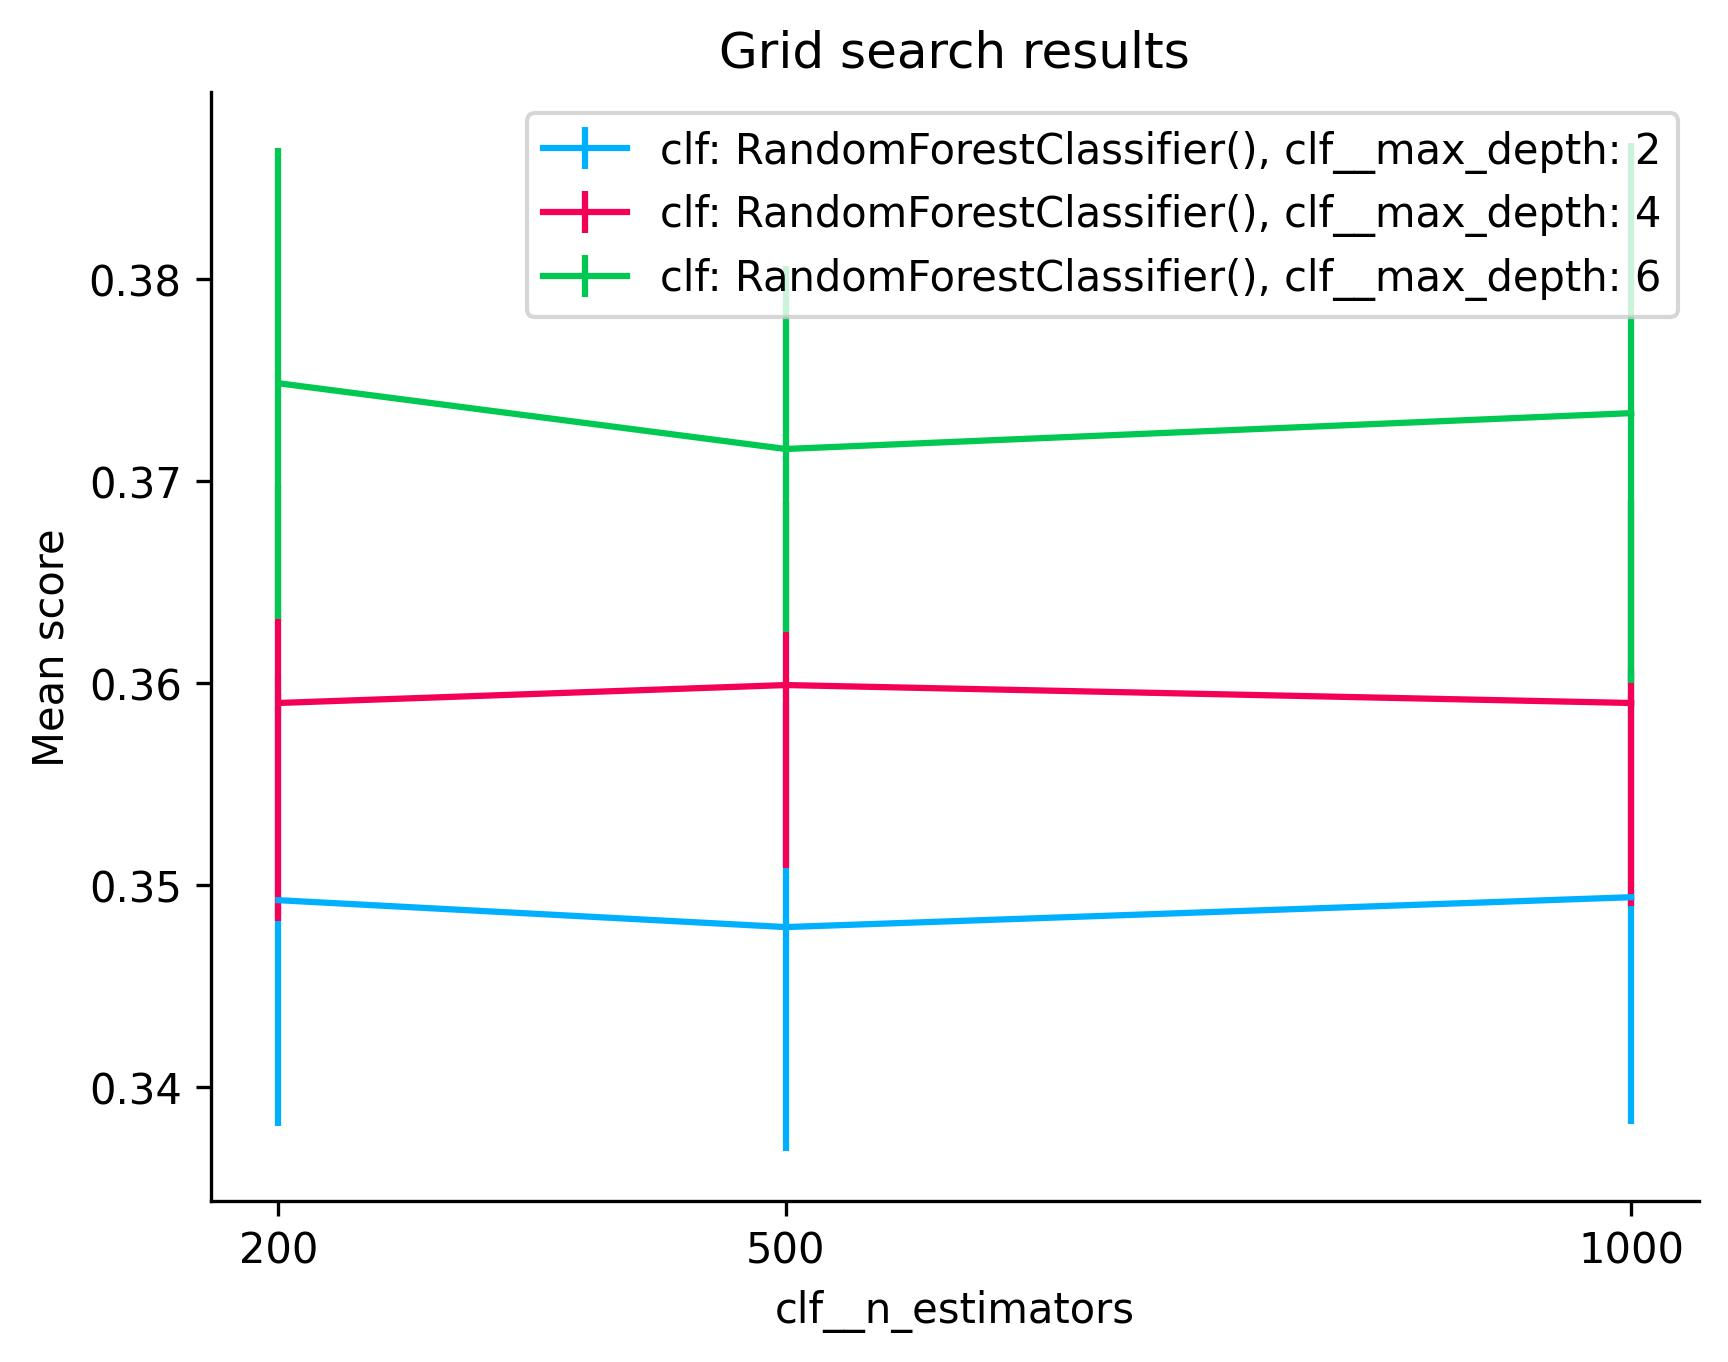
\includegraphics[width=\linewidth]{Graphs/GridSearch_rf_base.jpg}}
	\caption{figure 3 Example of a figure caption.}
	\label{GridSearch_rf_base}
\end{figure}
The baseline model had the best mean score at a max tree depth of 6 and 500 trees. Graphs for each of the models were made. The balanced class weight model had the best mean score with hyper parameters at a max tree depth of 4 and 500 trees. The imbalanced model had its best mean score with a max tree depth of 6 and 1000 trees. 

\subsection{Scoring}
Each of the 3 models were scored on both the training data and the testing data using a geometric mean score and classification matrix. Within the classification matrix the “zero” class is non arrests, the majority class, and the “one” class is arrests. The scoring of the models were compared and the best model was then selected. The testing data scoring is in the figures below in descending order of the baseline model, class weight balanced, and imbalanced model.
\begin{figure}[htbp]
	\centerline{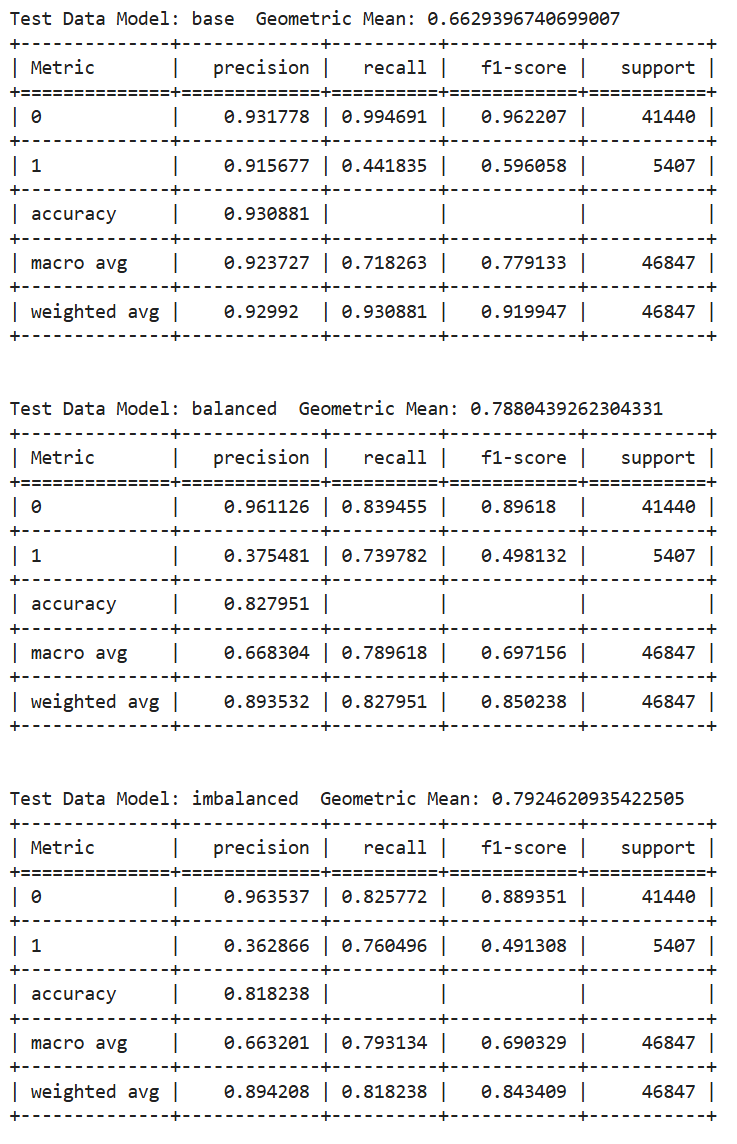
\includegraphics[width=\linewidth]{Graphs/Table_Graphs.png}}
	\caption{figure 3 Example of a figure caption.}
	\label{Table_Graphs}
\end{figure}

From the scoring we determined that the 3rd model, the imbalanced model performed the best. The imbalanced model has the highest geometric mean as well as the highest recall value for the arrest class. The precision values can often be misleading when dealing with imbalanced data. This is why we mainly looked at the geometric mean and recall. The recall value of the arrest classification was a key point as we want to maximize correct minority classification even if it means that the majority classifications suffer some. There is a higher cost to misclassify an arrest than to misclassify a non arrest. After determining that the imbalanced model performed the best according to our desired criteria, model interpretation methods were performed.

\subsection{Model Interpretation}
Feature importances and SHAP explainable learning was used to interpret our best model, the imbalanced model. Feature importance quantifies the level of importance or affect a particular data column has on the classification output. The feature importance values were graphed using a bar chart.
\begin{figure}[htbp]
	\centerline{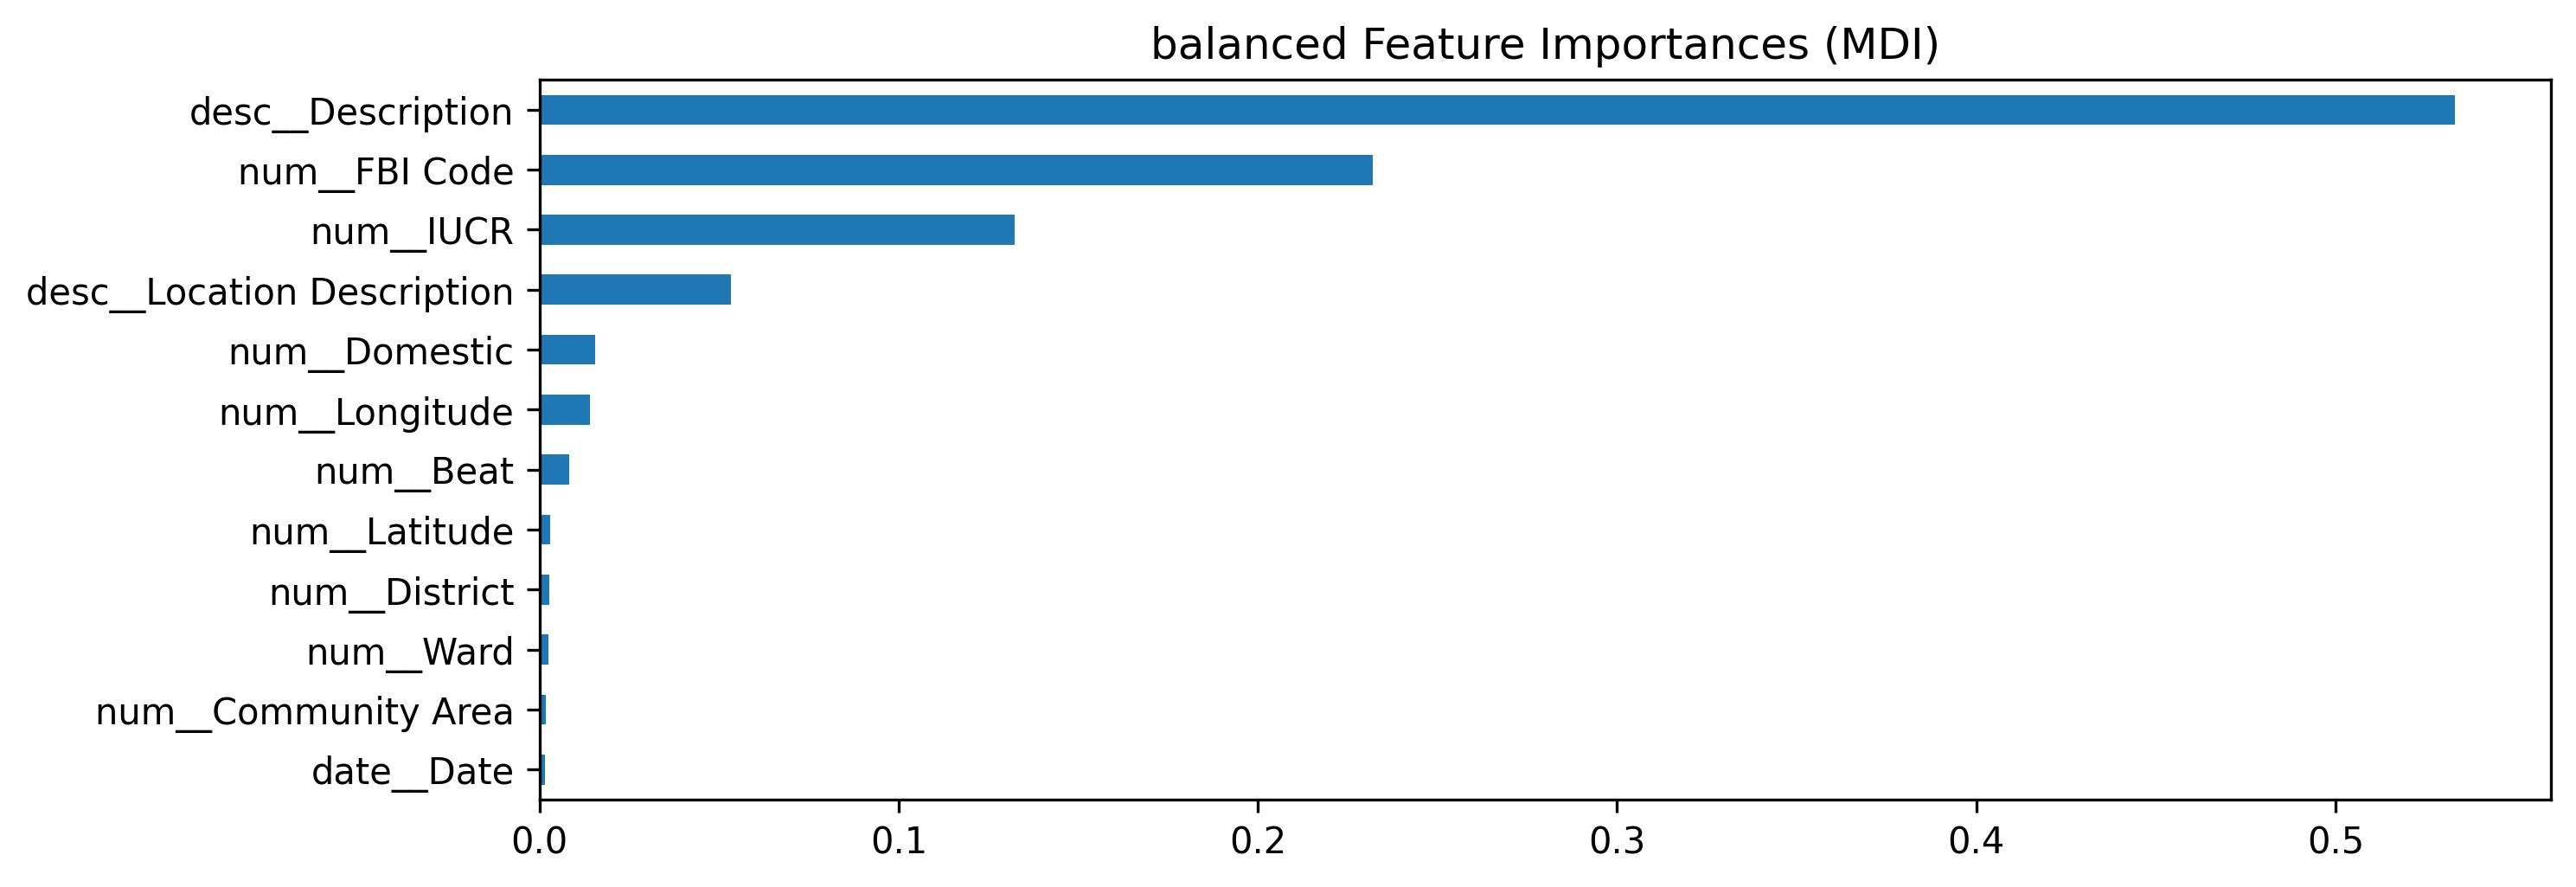
\includegraphics{Graphs/balanced_feature_importance.jpg}}
	\caption{figure 3 Example of a figure caption.}
	\label{balanced_feature_importance}
\end{figure}

From figure 5 it can be noted that only four columns had the majority of influence on classification. The crime description had the most importance then the corresponding FBI Code,  IUCR and then the location description. It may be considered unsurprising that the crime description had the largest importance, because the more egregious the crime the more likely law enforcement will focus on making those arrests. In addition to this the variable was target encoded, so the importance likely increased due to the type of encoding used.
SHAP explainable learning helped confirm our feature importance findings as well as explain how a prediction was made on the local level. SHAP explainable learning calculates Shapley values that are then used to describe how much a variable affects the classification including whether a high or low value impacts the classification positively or negatively.
\begin{figure}[htbp]
\centerline{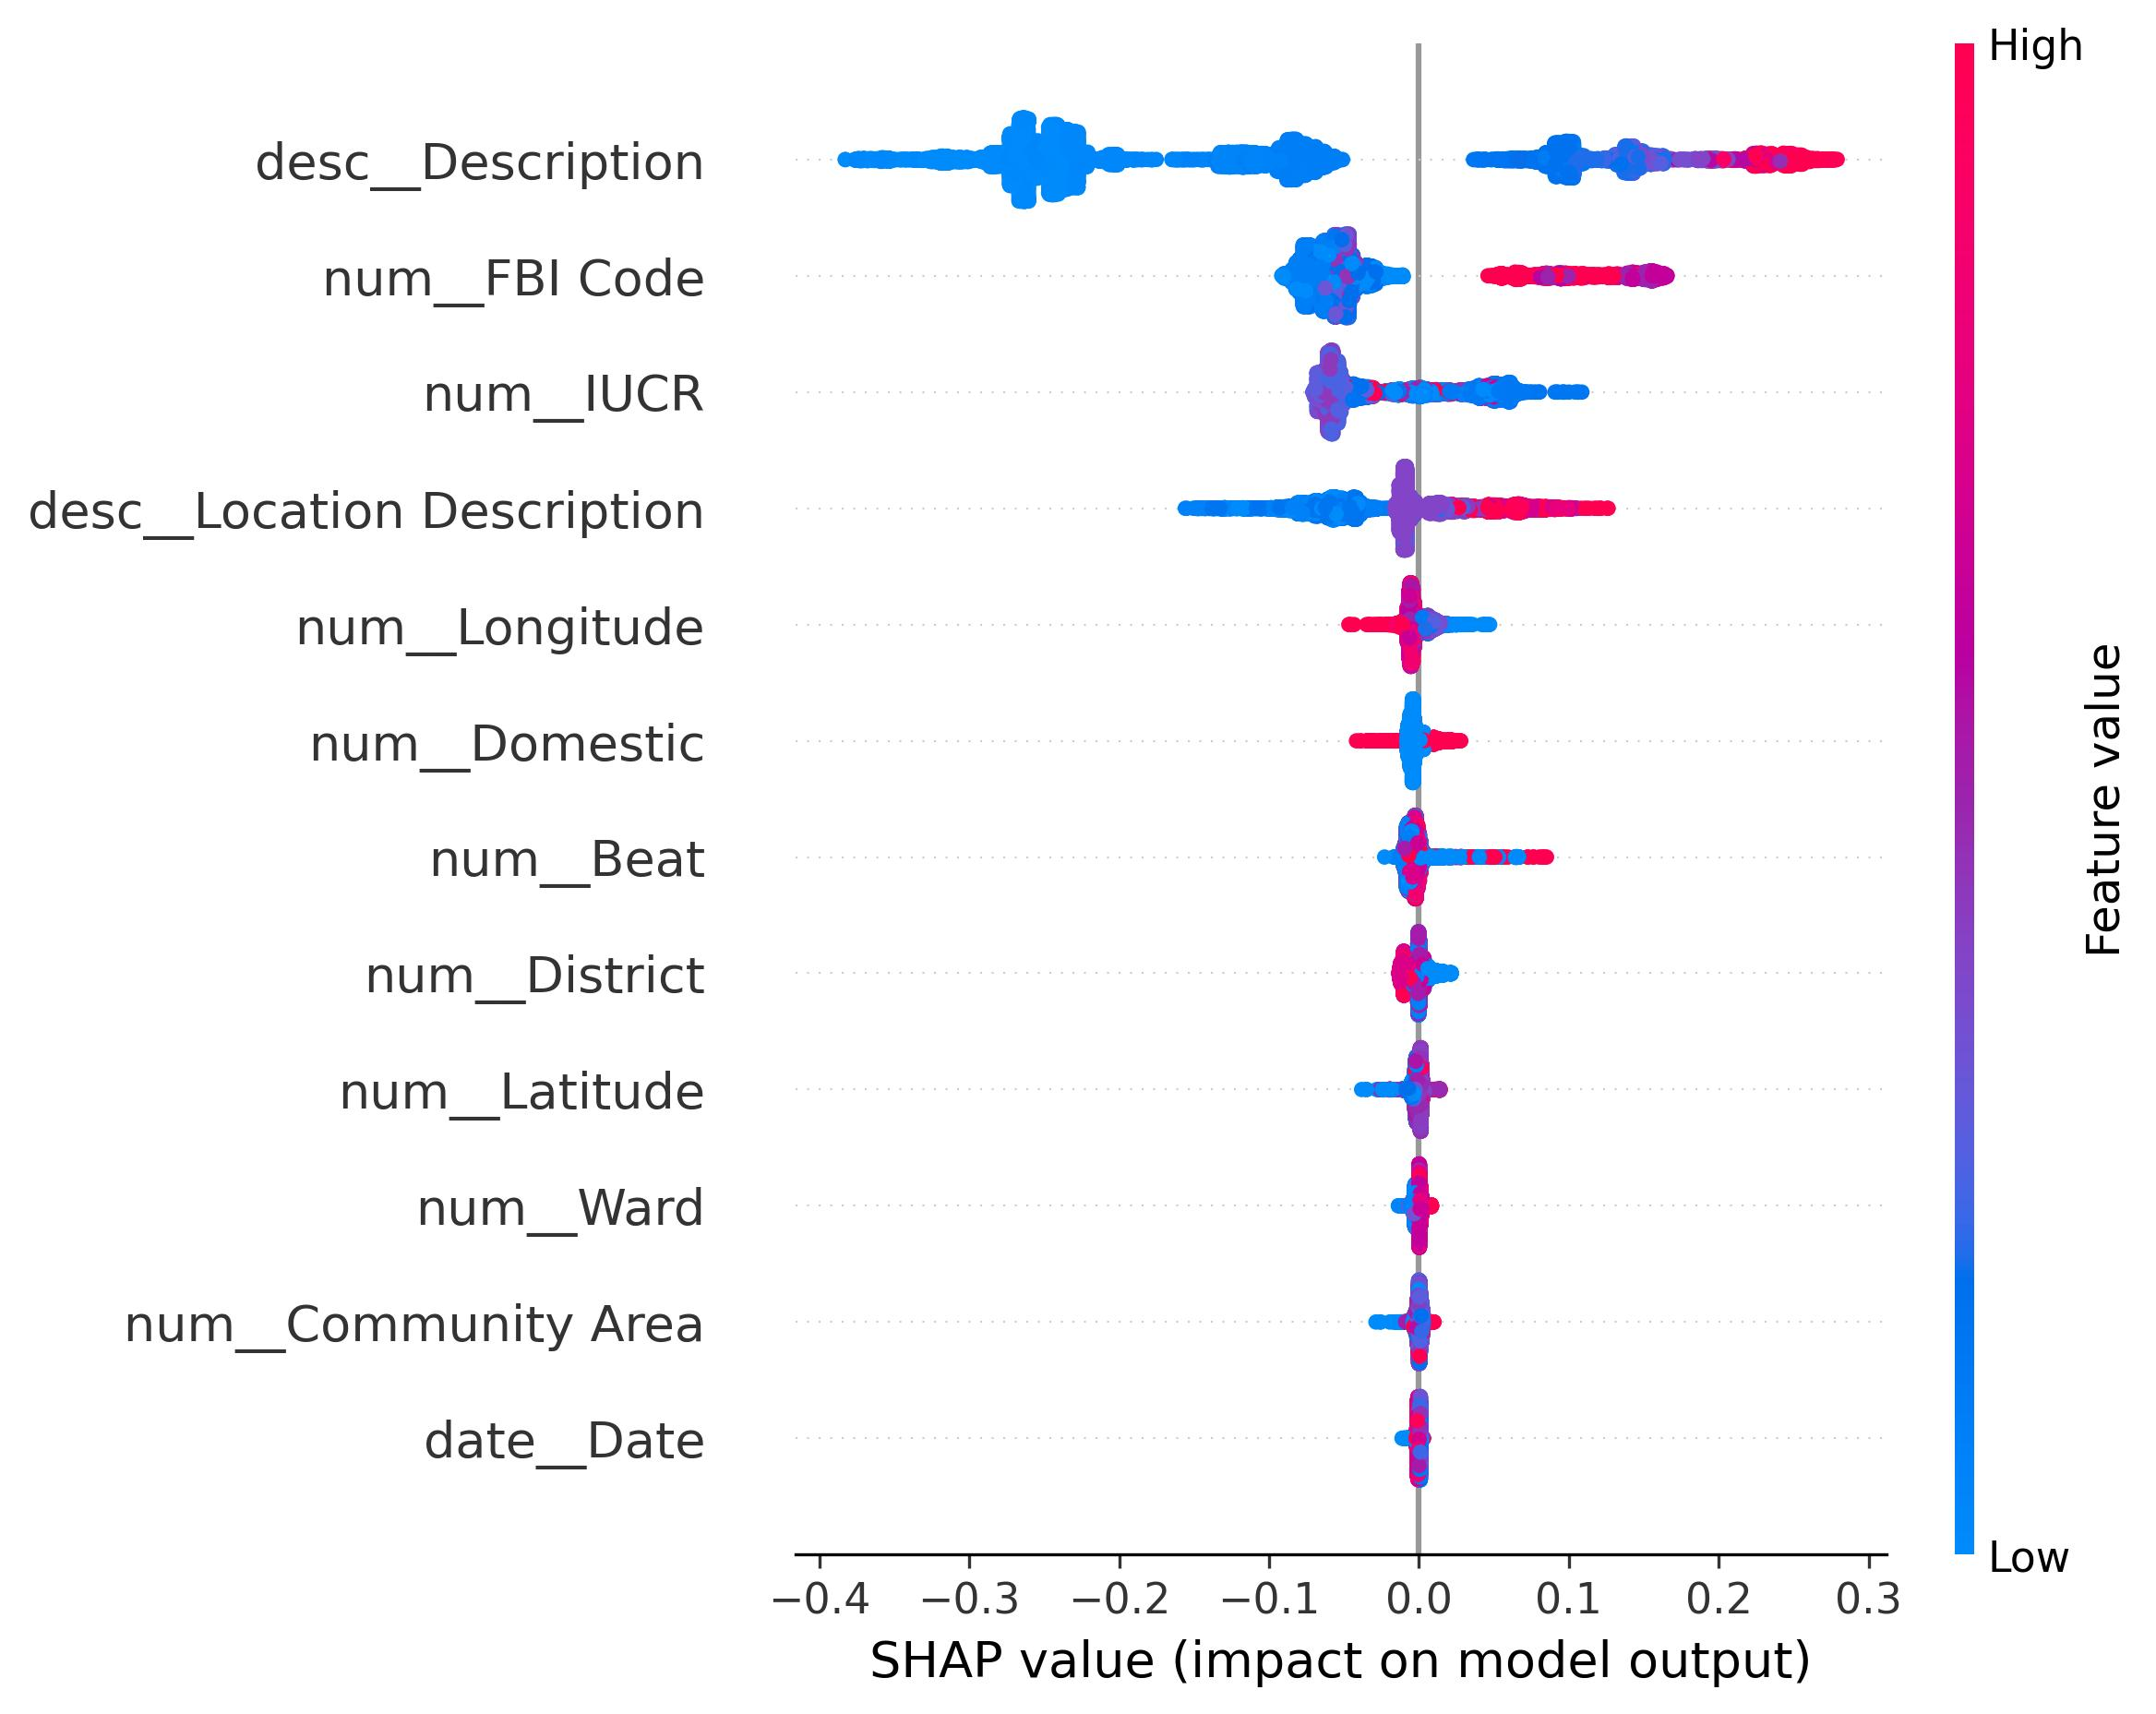
\includegraphics{Graphs/imbalanced_shap_impact.jpg}}
\caption{figure 3 Example of a figure caption.}
\label{imbalanced_shap_impact}
\end{figure}
Based on figure 6 we see that the same four features are at the top in importance level. It is hard to determine what a low or value of the description is due to the nature of its encoding making the SHAP plot less useful in this case. The FBI code and IUCR variables have similar difficulties as it is hard to know whether there is a pattern within the coding convention used. For example if a larger the value of FBI or IUCR code correlated to a more egregious crime we could use the SHAP plot to understand why those features contributed the way they did to classification. However, if there is no such correlation which is likely the case the SHApP plot can’t provide any additional information than feature importances.
SHAP explainable learning can be used to interpret local predictions. This is useful to understand why a particular prediction resulted in the classification of an arrest or non-arrest. A SHAP waterfall plot for an arrest and non-arrest will be shown below. 

\begin{figure}[htbp]
\centerline{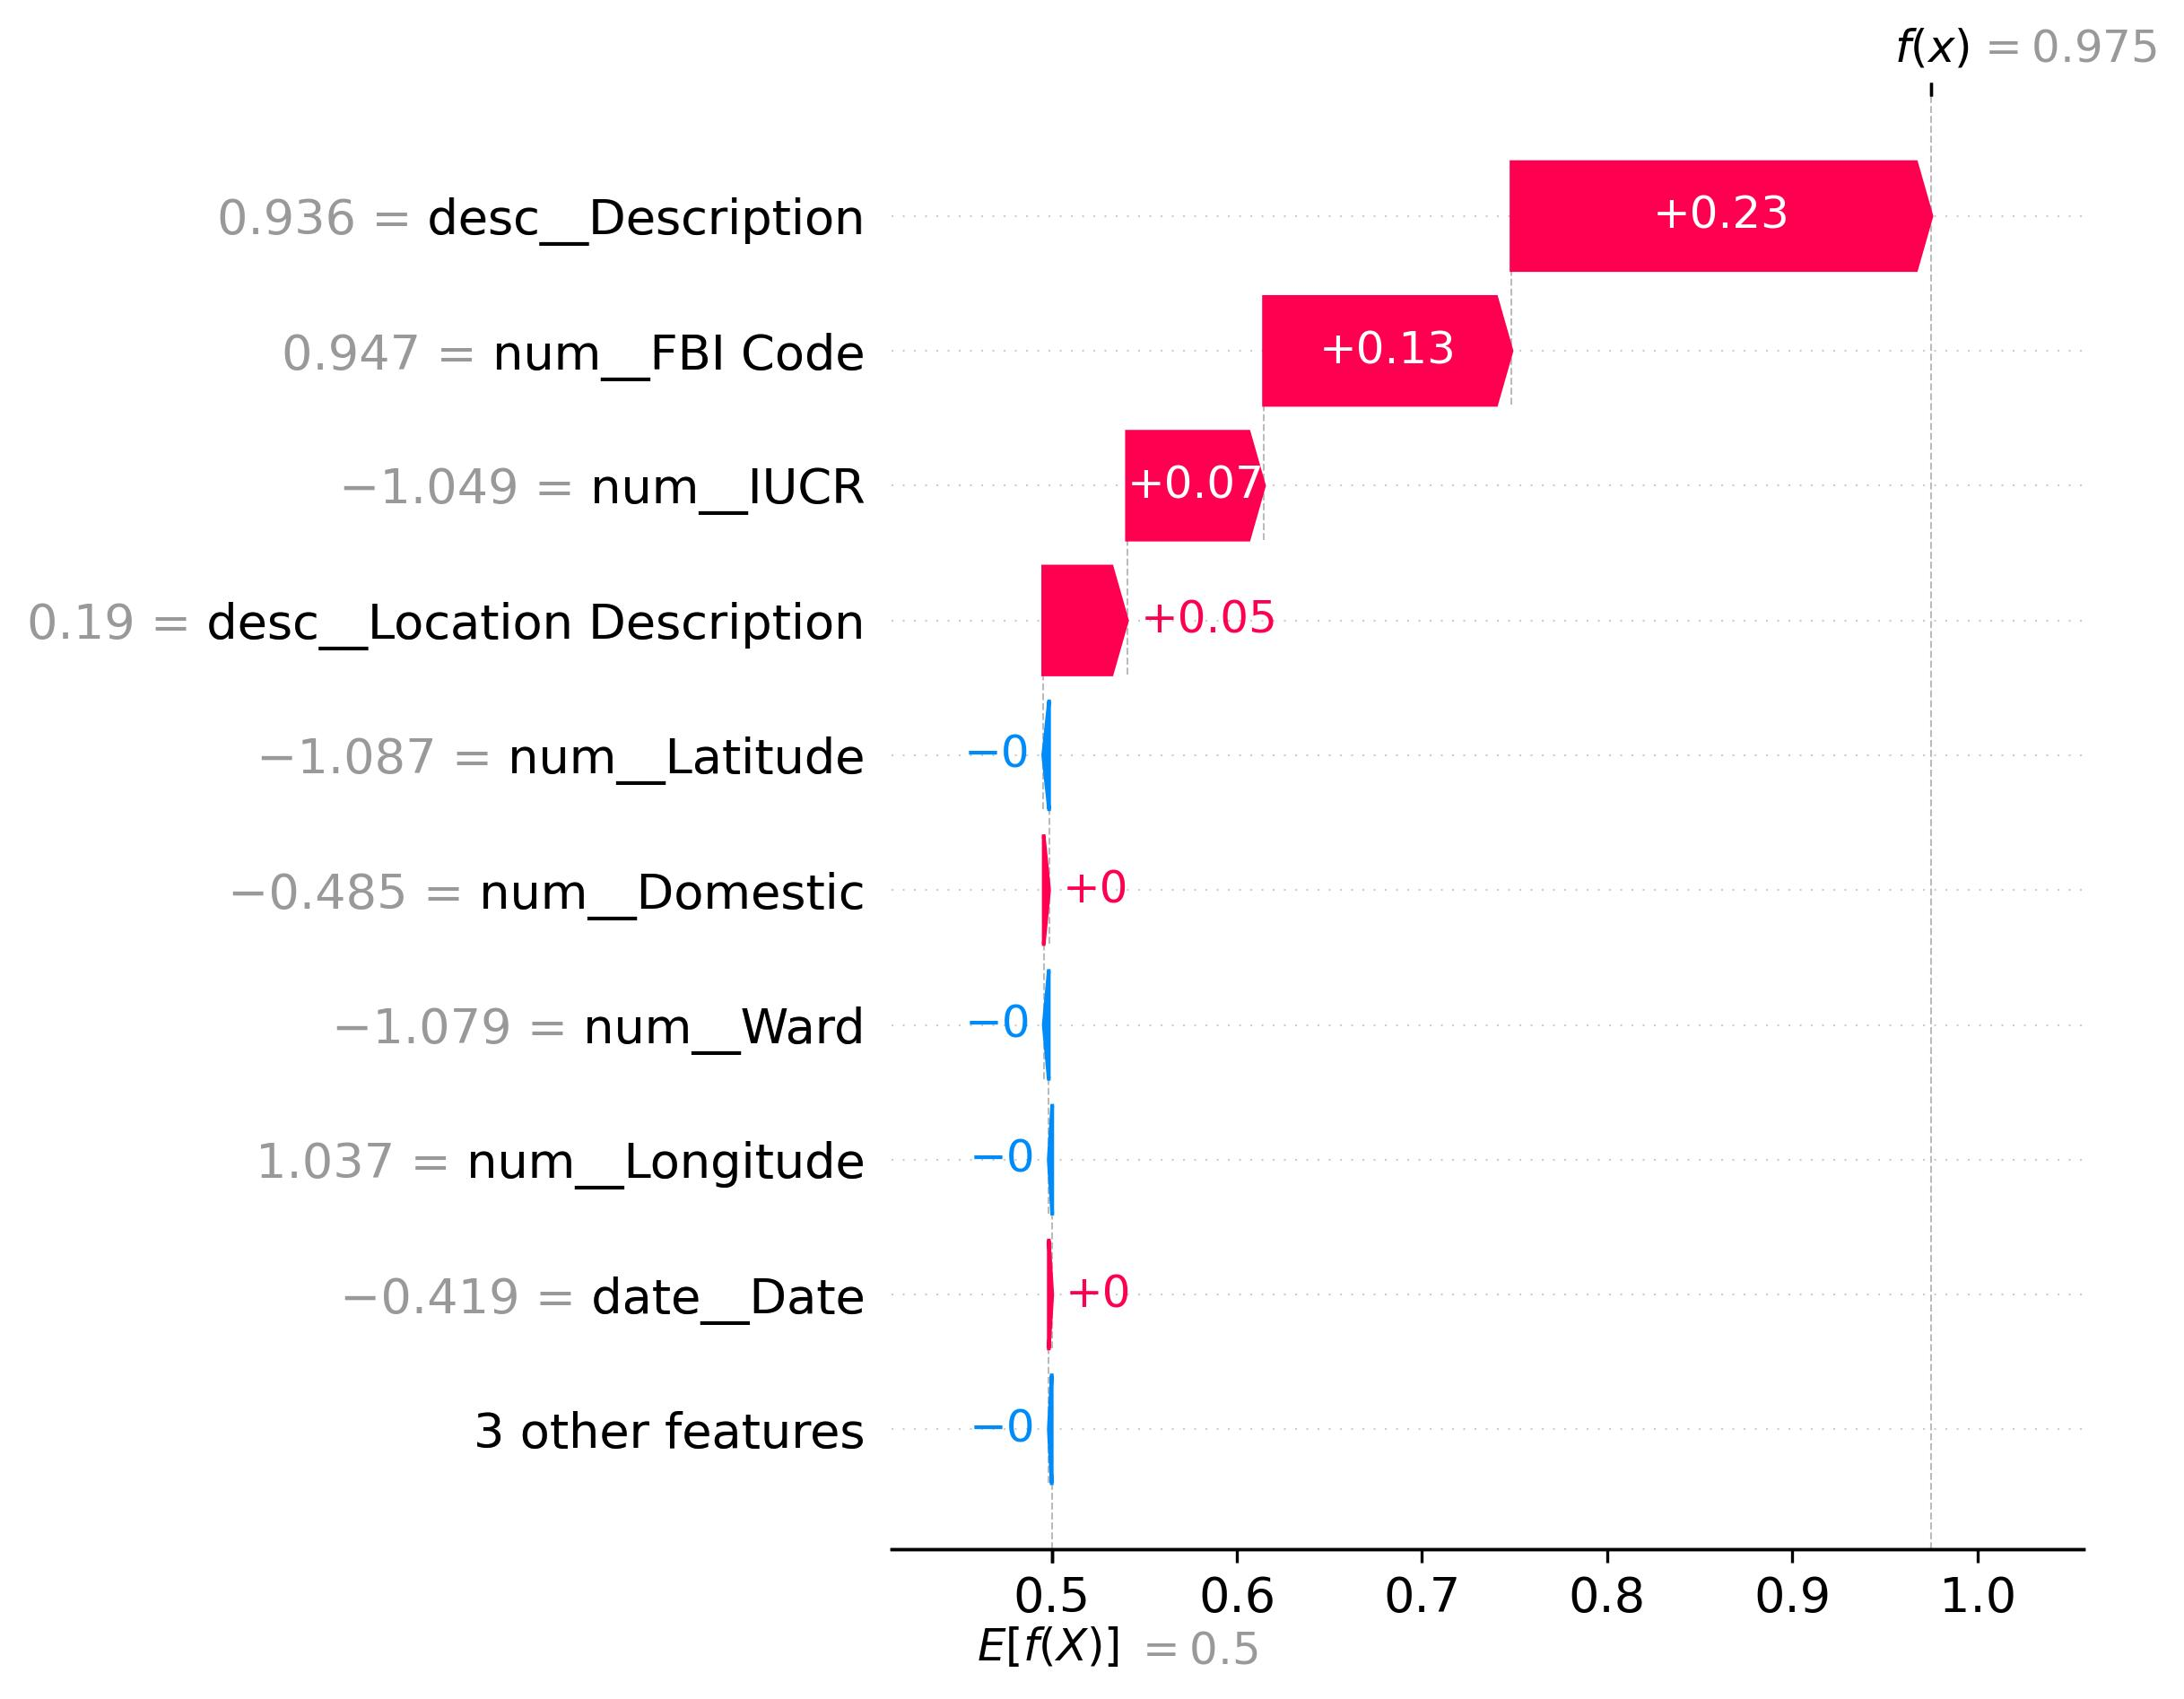
\includegraphics{Graphs/imbalanced_waterfall_plot/Details43.jpg}}
\caption{figure 3 Example of a figure caption.}
\label{figwaterfall3}
\end{figure}

\begin{figure}[htbp]
\centerline{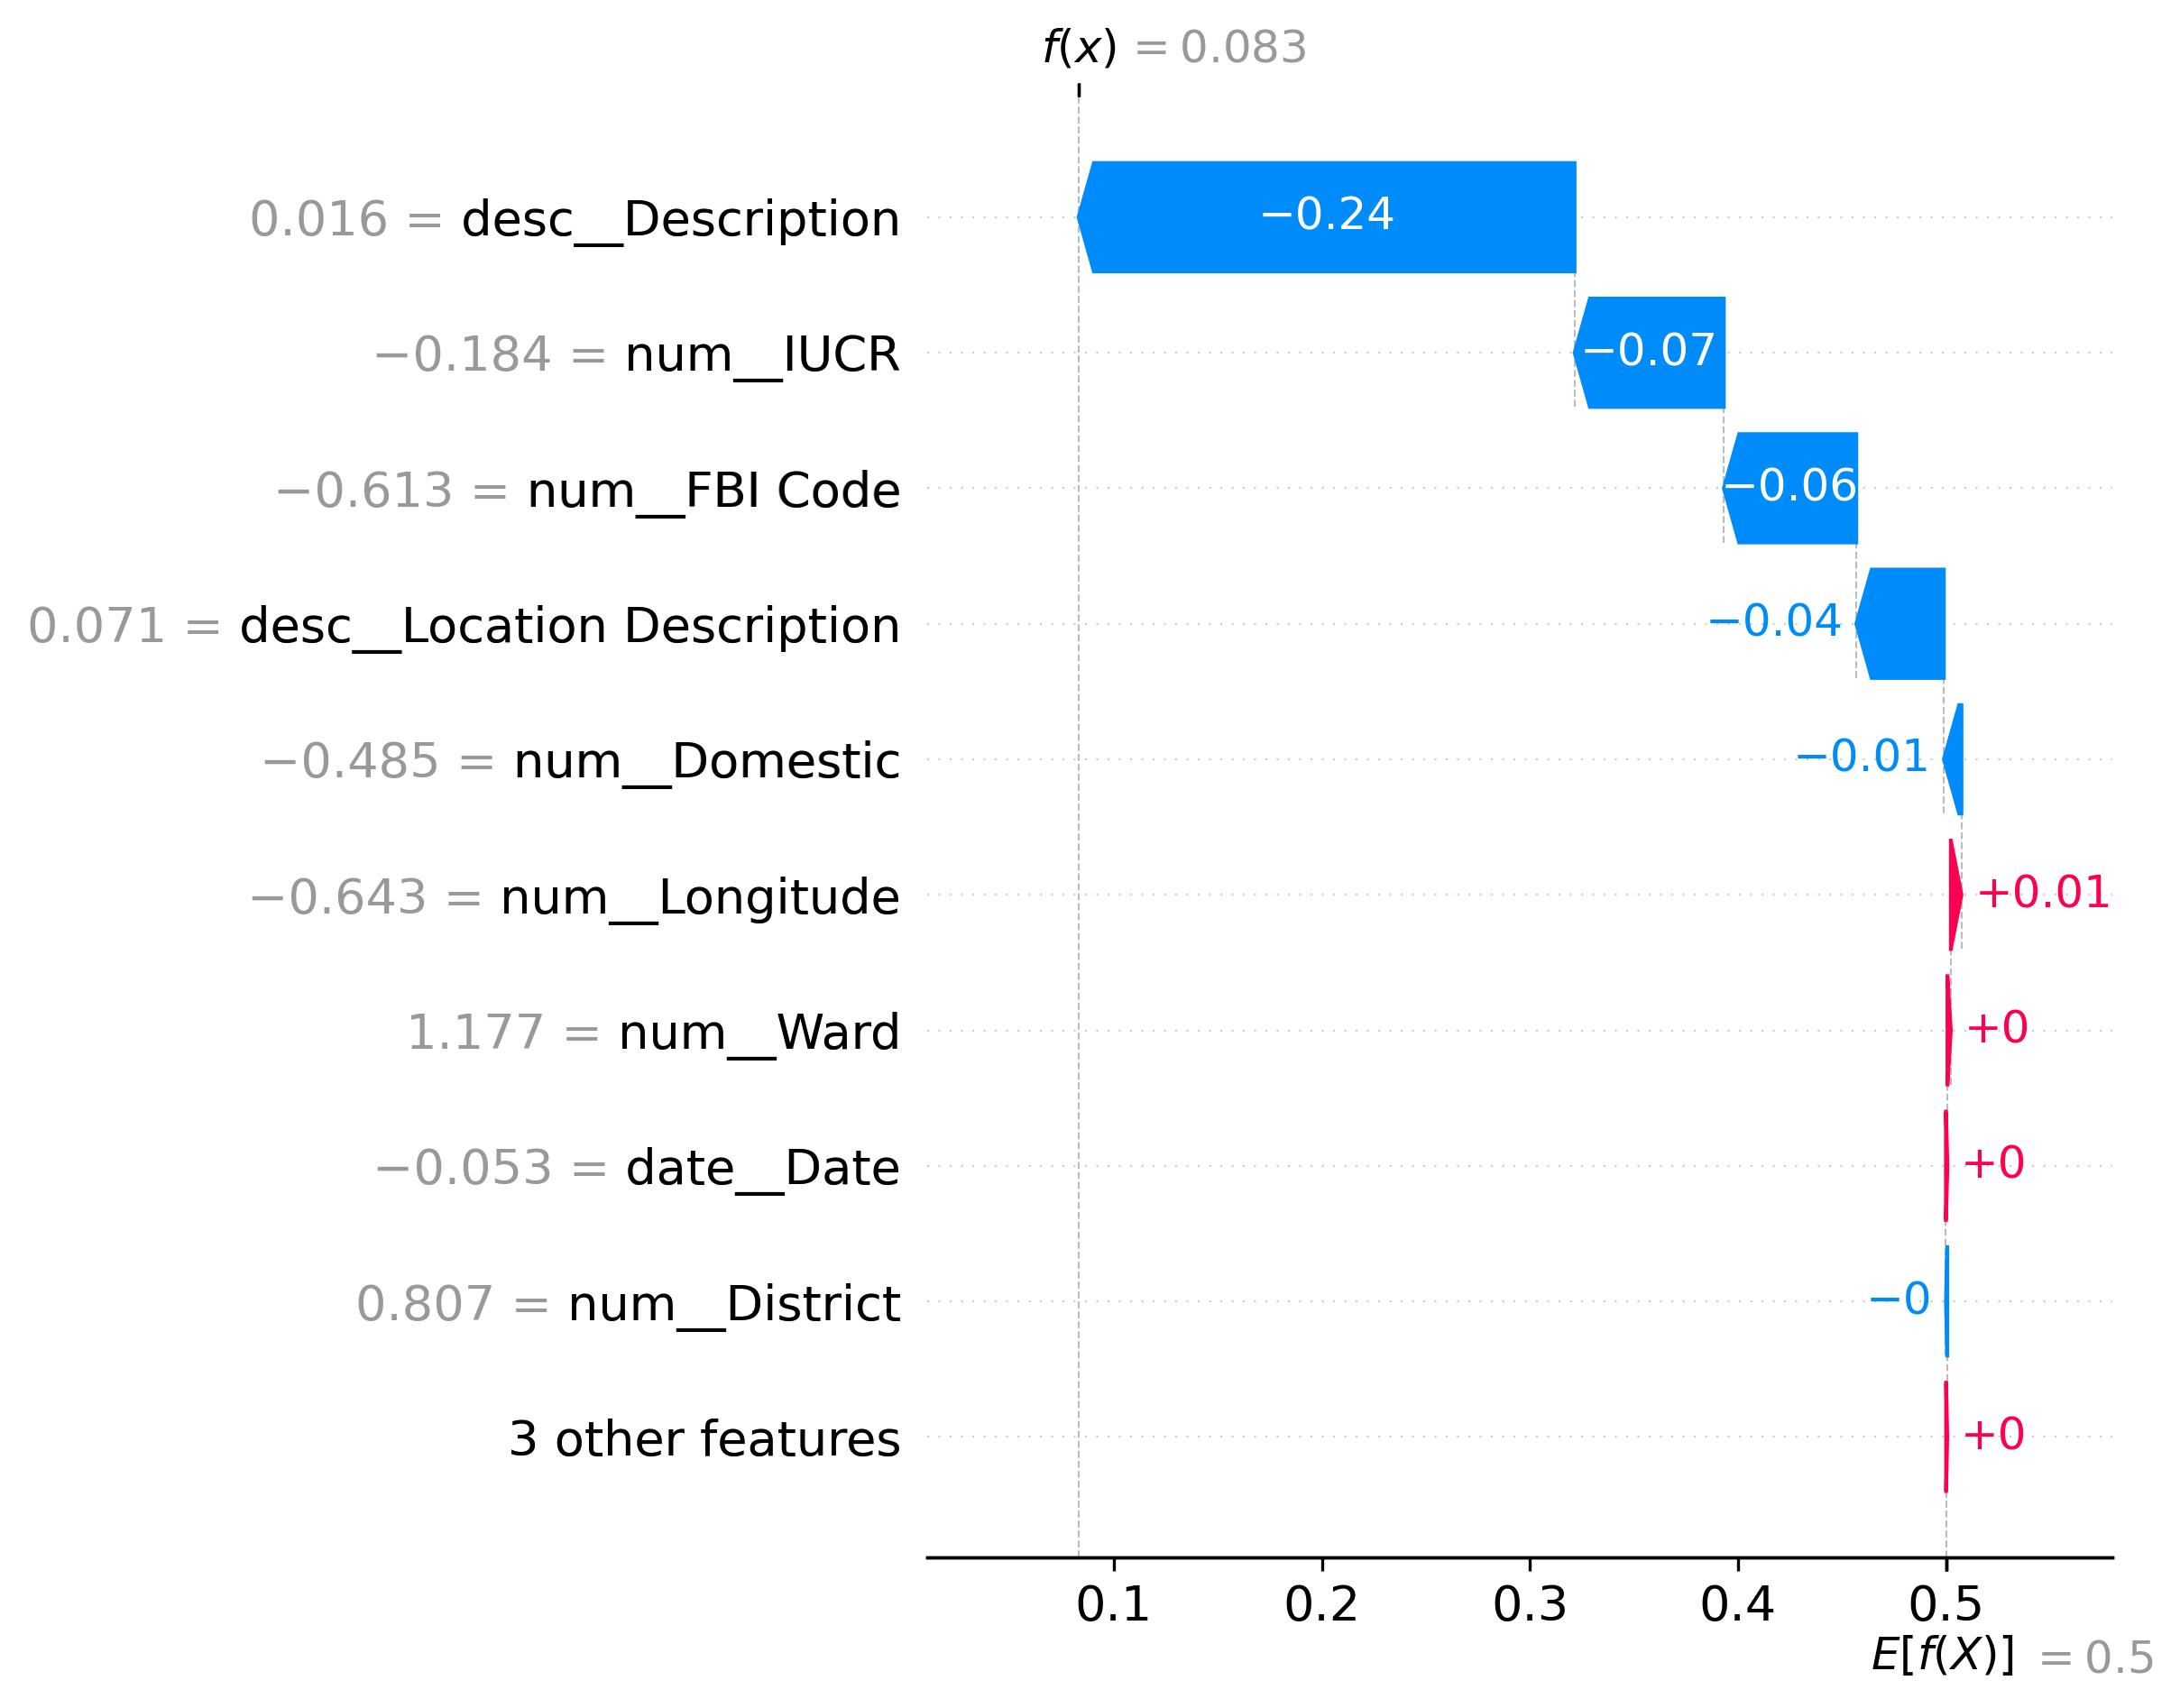
\includegraphics{Graphs/imbalanced_waterfall_plot/Details1.jpg}}
\caption{figure 3 Example of a figure caption.}
\label{figwaterfall1}
\end{figure}

Figure 7 is a SHAP waterfall plot for an arrest. It shows the quantification of each variable and its effect on the classification as an arrest. It's important to note that both figures 7 and 8 have value \begin{equation}
	E[f(x)]
	\end{equation}. That value is the initial value all predictions start at. It is at 0.5  due to the implementation of SMOTE and random undersampling for the imbalanced model. In the baseline model \begin{equation}
		E[f(x)]
		\end{equation} is 0.11 indication that the initial likelihood of being arrested is only 11\%.  The variables increase the likelihood of arrest in figure 7,m however in figure 8 the opposite is true. We have found that it is rare for the last 8 variables to make any significant contribution to the final likelihood.


\section{Conclusion}
The developed random forest classifier successfully predicted the likelihood of arrests using the Chicago Crimes-2022 dataset. Through comparative analysis, the imbalanced model emerged as the most effective due to its superior performance in geometric mean and recall scores, crucial for handling imbalanced data. Feature importance and SHAP explainability highlighted the significant impact of crime description, FBI code, IUCR, and location description on predictions. These findings not only validated the model's accuracy but also demonstrated its interpretability, enabling practical applications in law enforcement. Future work may involve incorporating additional features, optimizing encoding strategies, or extending the dataset to improve generalizability and operational utility.

\section*{Acknowledgment}
We extend our gratitude to the city of Chicago for providing access to the dataset and ensuring it remains up-to-date. Additionally, we sincerely thank Dr. Jishan Ahmed from Weber State University for his guidance in database projects and regression modeling. 

\section{Contributions}
\subsection{Coleton Watt}
Coleton Watt worked on finding the dataset. Working with SHAP and did the majority work on coding past the initial work by Dallin Baird. In this paper Coleton worked on section 3 and did the formatting. 
\subsection{Dallin Baird}
Dallin Baird did the initial work with cleaning the dataset, and building the primary models. He also managed and led creating the powerpoint presentation. Helped verify the results from SHAP and dictated what results were needed for the presentation. In this paper Dallin primarily worked on Results and Discussion.

\section*{References}

\begin{thebibliography}{00}
\bibitem{b1} https://github.com/Eleninja102/Math4750-Final-Project-Data-Modeling
\bibitem{b2} https://data.cityofchicago.org/Public-Safety/Crimes-2022/9hwr-2zxp/data 
\bibitem{b3} https://scikit-learn.org/stable/
\bibitem{b4} https://imbalanced-learn.org/stable/
\bibitem{b5} https://shap.readthedocs.io/en/latest/overviews.html
\bibitem{b6} https://data.cityofchicago.org/widgets/c7ck-438e 
\bibitem{b7} https://plotly.com/python/maps/ 
\bibitem{b8} https://geoffboeing.com/2014/08/clustering-to-reduce-spatial-data-set-size/ 
\bibitem{b9} https://medium.com/@khadijamahanga/using-latitude-and-longitude-data-in-my-machine-learning-problem-541e2651e08c
\bibitem{b10} https://data.cityofchicago.org/Public-Safety/Boundaries-Police-Beats-current-/aerh-rz74
\end{thebibliography}

\end{document}
